\chapter{Direct method: a reference for single scattering}
\label{ch:direct}

\section{Why a second method}

The Monte Carlo of the previous chapters reproduces the attenuation of the incident beam by \emph{where} the particles happen to interact: the
interaction points are drawn with the Beer--Lambert law. This is the natural way to follow particles through many scatterings, but for the
attenuation of \emph{singly} scattered particles it wastes most of the work when a layer attenuates weakly: in a 0.2~mm vanadium wall only about one
incident particle in a hundred interacts, and the other ninety-nine contribute nothing to that layer.

The module \code{direct_attenuation.py} computes the same single-scattering quantities in a different way, the \emph{direct} (or ``expected value'')
method. The attenuation is applied as an exact \emph{weight} instead of a random event, so every sample point contributes. The result is
\begin{itemize}
  \item a precise \textbf{reference} for the Monte Carlo results, to check them and to see their statistical scatter;
  \item the \textbf{Paalman \& Pings attenuation factors} of every layer, for any geometry of \mcams{} (slab or disc at any angle, cylinder, sphere, partially filled
        layers, beam profiles), with error bars;
  \item the exact expected \textbf{single-scattering intensity}, to put on top of the histograms of Chapter~\ref{ch:scattering}.
\end{itemize}
It does \emph{not} replace the Monte Carlo: it contains no multiple scattering, and for strongly attenuating samples the Monte Carlo is the more
efficient of the two (Section~\ref{sec:direct-efficiency}).

\section{The quantity computed}
\label{sec:direct-def}

For a layer $k$ and a scattering angle $\twotheta$, the \textbf{attenuation factor} is the average of the attenuation over the points $\mathbf r$ of the
material of the layer that are lit by the beam:
\begin{equation}
  A_k(\twotheta)=\frac{\displaystyle\int_{V_k} I(x,y)\,\exp\!\Big(-\sum_i\mu_i\big[L^{\mathrm{in}}_i(\mathbf r)+L^{\mathrm{out}}_i(\mathbf r,\twotheta)\big]\Big)\,\deriv V}
                     {\displaystyle\int_{V_k} I(x,y)\,\deriv V},
  \label{eq:Ak}
\end{equation}
where $I(x,y)=H(x)V(y)$ is the beam intensity, $L^{\mathrm{in}}_i$ the path in layer $i$ of the incident beam up to $\mathbf r$, and
$L^{\mathrm{out}}_i$ the path from $\mathbf r$ to the exit of the sample towards the detector. $A_k=1$ without attenuation. For a uniform beam and a
sample taller than the beam this is exactly the factor $A_{s,sc}$, $A_{c,sc}$, \dots{} of Paalman and Pings~\cite{pp}.

The second quantity is the \textbf{mean path} of the beam in the material of layer $k$, averaged over the whole beam (the parts that miss the layer
count as zero):
\begin{equation}
  \langle L_k\rangle=\frac{\int_{V_k} I(x,y)\,\deriv V}{\int_{\text{beam}} I(x,y)\,\deriv x\,\deriv y}.
\end{equation}
$\mu_k\langle L_k\rangle$ is the probability that an incident particle would interact in layer $k$ if there were no attenuation. With the scatter
fraction $f_k$, the singly scattered particles that leave the sample towards $\twotheta$, per incident particle and per steradian, are (isotropic
scattering)
\begin{equation}
  \frac{\deriv N_1}{N\,\deriv\Omega}(\twotheta)=\sum_k\frac{f_k\,\mu_k\,\langle L_k\rangle\,A_k(\twotheta)}{4\pi}.
  \label{eq:single-sr}
\end{equation}

\paragraph{Relation with the Monte Carlo.} \code{transmission_by_last_layer} (Chapter~\ref{ch:lastlayer}) adds up, for the first scatterings in
layer $k$, the outgoing attenuations. Because the interaction points already contain the incident attenuation, the expected value of that sum per
incident particle is $f_k\mu_k\langle L_k\rangle A_k(\twotheta)$. So the Monte Carlo gives the same $A_k$ after dividing by
$f_k\mu_k\langle L_k\rangle$; this is what \code{attenuation_factors_mc} does.

\section{How the direct method works}

\begin{figure}[ht]
\centering
\begin{tikzpicture}[scale=0.85]
  \fill[accent!8] (-5.2,-1.1) rectangle (4.5,1.1);
  \node[font=\small,color=ink2,anchor=west] at (-5.1,1.35) {beam};
  \draw[fill=accent!25,draw=accent] (0,0) circle (1.6);
  \draw[fill=accent2!25,draw=accent2] (0,0) circle (1.6) circle (1.85);
  \draw[fill=accent!25,draw=accent] (0,0) circle (1.6);
  \foreach \p in {(-0.9,0.5),(0.4,-0.7),(1.05,-0.15),(-0.3,-0.2),(-1.1,-0.35),(0.2,0.8),(1.68,-0.6),(-1.7,0.25)}
    \fill[ink2] \p circle (0.045);
  \fill[accent3] (0.5,0.45) circle (0.08);
  \draw[very thick,accent3,dashed] (-1.794,0.45) -- (0.5,0.45);  % from the outer surface (R = 1.85)
  \draw[very thick,accent3,-{Stealth[length=3mm]}] (0.5,0.45) -- ++(40:2.3);
  \draw[-{Stealth[length=3mm]},thick] (-5,0) -- (-3.3,0) node[midway,below,font=\small] {$+z$};
  \node[font=\small,accent3,anchor=south] at (-0.9,0.5) {$L^{\mathrm{in}}$};
  \node[font=\small,accent3,anchor=west] at (2.0,1.9) {$L^{\mathrm{out}}(\twotheta)$};
  \node[font=\small,anchor=west] at (0.62,0.2) {$\mathbf r$};
  \node[font=\small,accent2] at (1.95,-1.45) {can};
  \node[font=\small,accent] at (-0.15,-1.15) {sample};
\end{tikzpicture}
\caption{The direct method. Points (grey) are drawn uniformly in the volume lit by the beam and sorted by layer. For each point the incident path
(dashed, followed backwards from the point) and the outgoing path towards the detector are computed exactly; the point contributes the weight
$\exp[-\sum\mu(L^{\mathrm{in}}+L^{\mathrm{out}})]$.}
\label{fig:direct-sketch}
\end{figure}

\begin{enumerate}
  \item \textbf{Points.} $(x,y)$ is drawn from the beam profile (\code{sample_beam_point}) and $z$ uniformly over the extent of the sample along the beam.
        \code{layer_of_points} tells in which material the point is (points outside the material or in the empty part of a partially filled layer
        are discarded). The drawing goes on until every layer with $\mu>0$ has \code{n_points} points, so a thin wall gets as many points as the
        sample.
  \item \textbf{Incident path.} It is computed exactly by following the beam \emph{backwards} from the point to the surface of the sample:
        \code{outgoing_path_lengths(points, -z)}. This works for side faces, empty headspace and tilted slabs without any special case.
  \item \textbf{Outgoing path.} \code{outgoing_path_lengths(points, detector direction)} for every angle, as in Chapter~\ref{ch:transmission}.
  \item \textbf{Weights.} Each point contributes $w=\exp[-\sum_i\mu_i(L^{\mathrm{in}}_i+L^{\mathrm{out}}_i)]$. $A_k$ is the mean of the weights of
        layer $k$, and its error is their standard deviation divided by $\sqrt{n_k}$.
  \item \textbf{Mean paths.} $\langle L_k\rangle$ is estimated from an independent set of uniform points: the fraction $p$ of draws that fall in any
        material, and, for each point in the material, the full path of its beam line in each layer (backwards plus forwards), giving
        $\langle L_k\rangle=\Delta z\,p\,\langle L_k(\text{line})/L_{\mathrm{tot}}(\text{line})\rangle$. This ``ratio'' estimate is unbiased and
        much less noisy for thin layers than counting the points in each layer.
\end{enumerate}
Only methods of the common sample interface are used, so the direct method works for every geometry of \mcams{} and for any new one.

\section{Calling the functions}

\begin{lstlisting}
from direct_attenuation import (attenuation_factors_direct, attenuation_factors_mc,
                                compare_results, plot_attenuation_factors)

ref = attenuation_factors_direct(sample, beam_width, beam_height, H=None, V=None,
                                 angles_deg=None, phi_deg=0.0, n_points=200_000, rng=None)
mc  = attenuation_factors_mc(sample, beam_width, beam_height, H=None, V=None,
                             angles_deg=None, phi_deg=0.0, n_particles=200_000,
                             n_batches=5, mean_path=ref.mean_path, rng=None)
print(compare_results(ref, mc))           # table: values, difference, z
plot_attenuation_factors([ref, mc])       # lines: ref; points: mc; lower panel: difference
\end{lstlisting}

Both functions return an \code{AttenuationResult}:
\begin{center}\small
\begin{tabular}{@{}>{\raggedright\arraybackslash}p{5.4cm}p{9.2cm}@{}}
  \toprule \textbf{Attribute or method} & \textbf{Content} \\ \midrule
  \code{factors[k]}, \code{errors[k]} & $A_k(\twotheta)$ and its statistical error (one standard deviation), one row per layer; NaN for a layer
                                        with $\mu=0$ or not reached by the beam \\
  \code{mean_path}, \code{mean_path_error} & $\langle L_k\rangle$ (mm) and its error \\
  \code{single_per_steradian()} & equation~(\ref{eq:single-sr}): singly scattered particles per incident particle per steradian \\
  \code{angles_deg}, \code{layer_names}, \code{layer(name)} & the angles; the names of the layers; index of a layer from its name \\
  \code{n_samples}, \code{seconds}, \code{method} & points per layer (direct) or particles (MC); run time; \code{"direct"} or \code{"monte carlo"} \\ \bottomrule
\end{tabular}
\end{center}
\begin{itemize}
  \item \code{n_points} is the number of points \emph{per layer}. The error of $A_k$ decreases as $1/\sqrt{\text{\code{n_points}}}$;
        $10^5$ points give 0.02--0.2\,\% for $\mu R\le 0.5$.
  \item \code{attenuation_factors_mc} sets the scatter fractions to 1 in a copy of the sample (they do not change $A_k$) and runs
        \code{transmission_by_last_layer} with \code{max_orders=1}, in \code{n_batches} independent runs that give the error bars. Give it
        \code{mean_path=ref.mean_path}, or the exact value when you know it (uniform beam lower than a cylindrical sample: area of the layer inside the
        beam divided by the beam width); otherwise it is estimated with \code{mean_material_paths}.
  \item \code{mean_material_paths(sample, beam_width, beam_height, H, V)} alone returns $\langle L_k\rangle$ and its error.
\end{itemize}

\pyexample{ex09_direct}

The thin V wall shows the difference between the methods: $10^5$ points give $A_{\mathrm V}$ to 0.15\,\% with the direct method, while
$2\times10^5$ Monte Carlo particles give 3\,\%.

\section{Using it as a reference for the Monte Carlo}

\subsection{Attenuation factors}

Run both functions with the same sample, beam and angles and look at \code{compare_results}: the column \code{z} is the difference in units of the
combined statistical error. If the two methods agree, $|z|$ is below 2 for most angles and layers and almost never above 3
(Figure~\ref{fig:direct-vs-mc}). Remember that the Monte Carlo uses the same particles for all angles, so its errors at different angles are
correlated: a whole curve may be shifted by about one error bar.

\begin{figure}[ht]
  \centering
  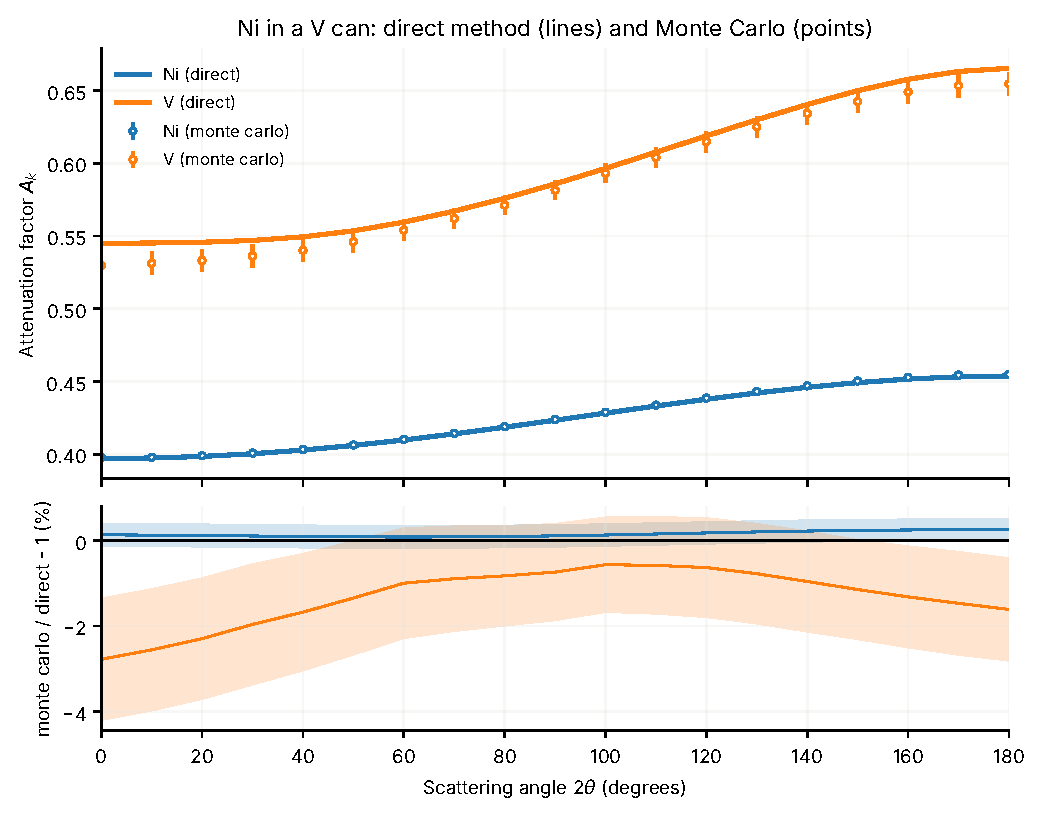
\includegraphics[width=0.82\textwidth]{fig_direct_vs_mc}
  \caption{Ni rod (6~mm) in a V can (0.2~mm), beam $15\times20$~mm: attenuation factors from the direct method (lines,
  $2\times10^5$ points per layer) and from the Monte Carlo (points, $20\times25\,000$ particles). Lower panel: relative difference with its
  $1\sigma$ band. The Monte Carlo error of the thin V wall is ten times larger than that of the direct method.}
  \label{fig:direct-vs-mc}
\end{figure}

\subsection{Single-scattering counts}

The particle-by-particle simulation of Chapter~\ref{ch:scattering} gives the singly scattered particles per steradian. Its expected value is
equation~(\ref{eq:single-sr}), which the direct method gives without noise. The detector direction of the direct method lies in the horizontal plane,
so use a narrow azimuth window in the simulation:
\begin{lstlisting}
from multiple_scattering import simulate_scattering_orders
res = simulate_scattering_orders(sample, 15, 20, n_particles=16_000_000,
                                 angle_edges_deg=np.arange(0, 181, 5.0),
                                 phi_deg=0.0, phi_halfwidth_deg=5.0, rng=7)
ref = attenuation_factors_direct(sample, 15, 20, angles_deg=res.angles_deg)
single_mc  = res.per_steradian(res.single)
single_ref = ref.single_per_steradian()          # the exact expectation
multiple   = res.per_steradian(res.multiple)     # Monte Carlo only
\end{lstlisting}

\begin{figure}[ht]
  \centering
  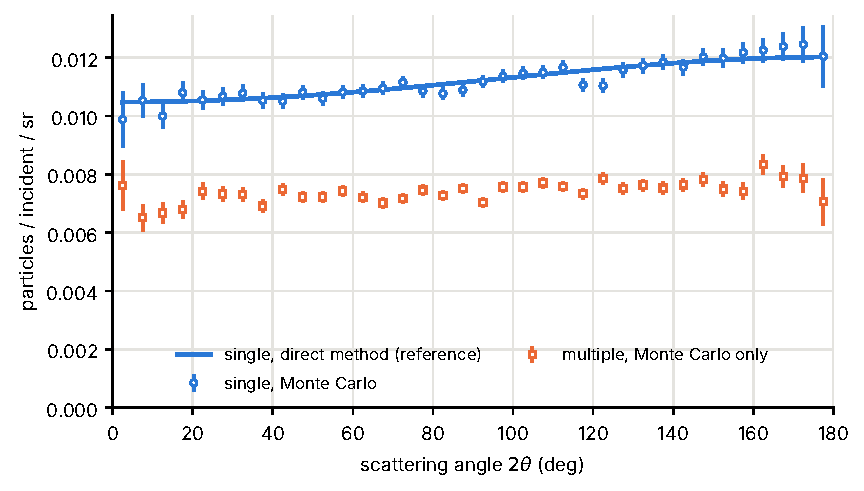
\includegraphics[width=0.78\textwidth]{fig_direct_orders}
  \caption{Same sample, $1.6\times10^7$ particles, azimuth window $\pm5^\circ$, $5^\circ$ bins. The single-scattering counts of the Monte Carlo
  (blue points) follow the direct reference (line): $\chi^2$ per bin 0.67, mean difference $-0.13\,\%$. The multiple scattering (orange) has
  no direct equivalent.}
  \label{fig:direct-orders}
\end{figure}

This comparison checks the whole random walk of the first event (beam, interaction point, scattering, direction, exit, counting) against an
independent calculation, and it separates in the measured signal the part that is known precisely (single) from the part that only the Monte Carlo
gives (multiple).

\section{Accuracy of the direct method}

The direct method has no discretisation: the paths are exact, and its only error is statistical and is computed with the result. It was checked
against exact or deterministic results (script \file{tools/direct\_method\_analysis.py}, part~1, $4\times10^5$ points per layer):

\begin{table}[H]
  \centering\small
  \begin{tabular}{@{}>{\raggedright\arraybackslash}p{6.2cm}ccccc@{}}
    \toprule \textbf{Case} & $\twotheta$ & \textbf{exact} & \textbf{direct} & \textbf{error} & $z$ \\ \midrule
    Slab, $\mu t=0.5$ (analytic) & $0^\circ$   & 0.60653 & 0.60653 & 0       & exact \\
                                                   & $60^\circ$  & 0.47730 & 0.47732 & 0.00011 & 0.15 \\
                                                   & $150^\circ$ & 0.61215 & 0.61212 & 0.00030 & $-0.12$ \\
    Same slab, fullness 0.5                        & $150^\circ$ & 0.61215 & 0.61265 & 0.00030 & 1.66 \\
    Ni + V can, 2~mm beam, $A_s$ (1D integral) & $0^\circ$ & 0.33956 & 0.33956 & 0.00001 & $-0.08$ \\
                                                   & $180^\circ$ & 0.40701 & 0.40752 & 0.00038 & 1.32 \\
    Furnace, $A_{h,sch}$ (fine grid) & $30^\circ$  & 0.75307 & 0.75316 & 0.00042 & 0.22 \\
                                                   & $150^\circ$ & 0.76136 & 0.76130 & 0.00044 & $-0.13$ \\ \bottomrule
  \end{tabular}
  \caption{Direct method against exact results: slab (analytic formulas for transmission and reflection), cylinder at $0^\circ$ and $180^\circ$
  (where the 2D integral reduces to a 1D integral, computed with \code{scipy.integrate.quad}) and a furnace at the angles where its factor has deep
  minima (deterministic midpoint grid of $40\times80\,000$ points, converged). $z$ = difference / error.}
  \label{tab:direct-exact}
\end{table}

All the differences are within the statistical error. The mean path is also correct: $\langle L\rangle=2.0000$~mm for the full slab of 2~mm and,
over 20 independent runs, $1.00003\pm0.00023$~mm for the slab filled to half the beam height (exact: 1~mm); the error quoted by the function
(0.00100 per run) agrees with the scatter of the runs (0.00104).

\section{Direct method and Monte Carlo compared}
\label{sec:direct-efficiency}

\subsection{Agreement}

Four samples were computed with both methods (part~2 of the script; direct: $2\times10^5$ points per layer, Monte Carlo: $20\times25\,000$
particles, 19 angles):

\begin{table}[H]
  \centering\small
  \begin{tabular}{@{}>{\raggedright\arraybackslash}p{4.4cm}lccccc@{}}
    \toprule \textbf{Sample} & \textbf{layer} & max$|z|$ & \textbf{mean diff.} & \textbf{err.\ direct} & \textbf{err.\ MC} & \textbf{FOM d/MC} \\ \midrule
    Ni in V can, 15~mm beam & Ni & 1.00 & $+0.15$\,\% & 0.09\,\% & 0.25\,\% & 1.7 \\
                                      & V  & 1.94 & $-1.32$\,\% & 0.11\,\% & 1.27\,\% & 30 \\
    same, 2~mm beam                   & Ni & 0.40 & $-0.02$\,\% & 0.08\,\% & 0.14\,\% & 2.0 \\
                                      & V  & 0.23 & $+0.13$\,\% & 0.10\,\% & 1.63\,\% & 148 \\
    Slab Al/Fe/Cu at $60^\circ$ & Al & 0.34 & $-0.13$\,\% & 0.02\,\% & 0.74\,\% & 580 \\
                                      & Fe & 0.86 & $-0.11$\,\% & 0.03\,\% & 0.27\,\% & 18 \\
                                      & Cu & 1.29 & $-0.27$\,\% & 0.02\,\% & 0.35\,\% & 55 \\
    Powder, $f=0.6$ & powder & 1.67 & $-0.41$\,\% & 0.12\,\% & 0.25\,\% & 1.3 \\
                                      & V  & 1.03 & $+0.84$\,\% & 0.11\,\% & 1.09\,\% & 30 \\ \bottomrule
  \end{tabular}
  \caption{Direct method against Monte Carlo (beam heights: 20~mm for the cylinders, 8~mm for the others; the powder fills its can to 0.6 of the beam height, in a Gaussian beam profile). max$|z|$: largest difference over the angles in units of the combined error; mean diff.: average
  of MC/direct\,$-1$ over the angles (correlated, see text); err.: mean relative error; FOM: figure of merit, defined below.}
  \label{tab:direct-mc}
\end{table}

The two methods agree within the statistics in every case, including the tilted slab, the partially filled container and the non-uniform beam
($|z|<2$ everywhere). The ``mean differences'' of about 1\,\% for the V walls are one correlated Monte Carlo error bar: the whole MC curve moves
together.

\subsection{Efficiency}

The \textbf{figure of merit} $\mathrm{FOM}=1/(\varepsilon^2\,t)$, with $\varepsilon$ the relative error and $t$ the run time, does not depend on the
number of samples: a method with ten times the FOM reaches the same precision ten times faster. Figure~\ref{fig:direct-fom} shows the ratio of the
FOM of the two methods for a single full cylinder ($R=3$~mm, beam $8\times20$~mm) as a function of its attenuation $\mu R$ (part~3 of the script):

\begin{figure}[ht]
  \centering
  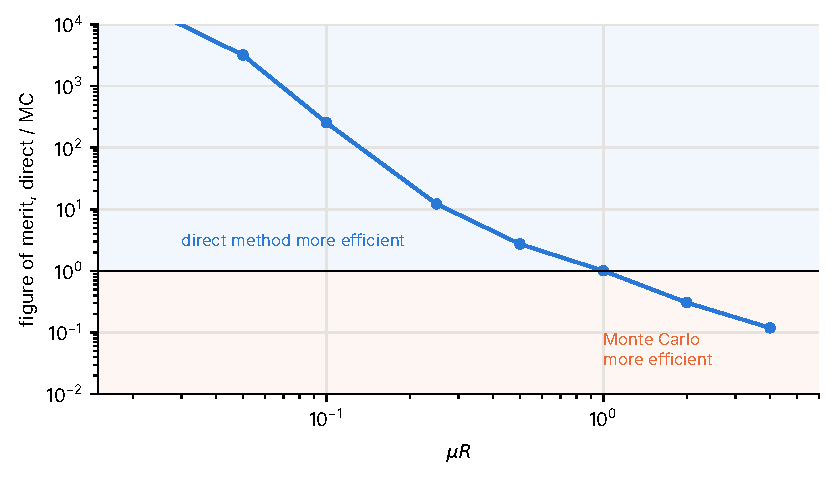
\includegraphics[width=0.72\textwidth]{fig_direct_fom}
  \caption{Figure of merit of the direct method divided by that of the Monte Carlo, for a cylinder of radius 3~mm, versus $\mu R$.}
  \label{fig:direct-fom}
\end{figure}

\begin{table}[H]
  \centering\small
  \begin{tabular}{@{}cccccc@{}}
    \toprule $\mu R$ & $A(90^\circ)$ & \textbf{interacting fraction} & \textbf{err. direct} & \textbf{err. MC} & \textbf{FOM direct/MC} \\ \midrule
    0.02 & 0.967 & 0.023 & 0.005\,\% & 0.91\,\% & 28\,000 \\
    0.05 & 0.919 & 0.056 & 0.011\,\% & 0.73\,\% & 2\,800 \\
    0.10 & 0.846 & 0.108 & 0.023\,\% & 0.39\,\% & 240 \\
    0.25 & 0.665 & 0.240 & 0.057\,\% & 0.19\,\% & 13 \\
    0.50 & 0.458 & 0.399 & 0.116\,\% & 0.16\,\% & 2.6 \\
    1.00 & 0.243 & 0.575 & 0.236\,\% & 0.16\,\% & 0.86 \\
    2.00 & 0.100 & 0.695 & 0.495\,\% & 0.17\,\% & 0.26 \\
    4.00 & 0.040 & 0.738 & 1.06\,\%  & 0.24\,\% & 0.12 \\ \bottomrule
  \end{tabular}
  \caption{Same comparison in numbers: direct method $10^5$ points, Monte Carlo $20\times25\,000$ particles, 5 angles. The agreement is within
  $|z|<1.6$ at all $\mu R$.}
  \label{tab:direct-fom}
\end{table}

\paragraph{Why.} The two methods treat the incident attenuation in opposite ways.
\begin{itemize}
  \item The \textbf{Monte Carlo} places its interaction points with the Beer--Lambert law: where the beam is strong. This is \emph{importance
        sampling} of the incident attenuation, and the only remaining randomness is the outgoing attenuation. Its weakness is that only the
        interacting fraction of the particles (third column) does any work: for $\mu R=0.02$, 98\,\% of them cross the sample and are wasted.
  \item The \textbf{direct method} uses every point, but weights it with the incident attenuation. When the attenuation is weak the weights are all
        close to one and the variance is tiny. When it is strong the weights span orders of magnitude (most points sit in the ``shadow'' and carry
        almost nothing), and a few points near the entrance surface dominate the mean.
\end{itemize}
The two are equally efficient near $\mu R\approx1$ (more precisely, when about half of the beam interacts in the layer).

\section{When to use which}

\begin{table}[H]
  \centering\small
  \begin{tabular}{@{}>{\raggedright\arraybackslash}p{7.4cm}>{\raggedright\arraybackslash}p{7.2cm}@{}}
    \toprule \textbf{Situation} & \textbf{Best tool} \\ \midrule
    Attenuation factors of containers, furnace and cryostat walls, thin layers, weakly absorbing samples ($\mu R\lesssim0.5$) &
      \textbf{direct method}: 10 to $10^4$ times faster at equal precision \\
    Attenuation factors of a typical sample, $\mu R\approx0.5$--1 & either; the direct method is simpler (no normalisation) \\
    Attenuation factors of strongly attenuating samples, $\mu R\gtrsim1$ & \textbf{Monte Carlo}: 4--8 times more efficient at $\mu R=2$--4 \\
    Multiple scattering, scattering orders, last layer of multiply scattered particles & \textbf{Monte Carlo only} \\
    Effect of the angular distribution of the scattering (Henyey--Greenstein, \dots) & \textbf{Monte Carlo only} (single attenuation does not
      depend on it) \\
    Histograms with bins and azimuth windows, total measured signal & \textbf{Monte Carlo}; the direct method gives the exact single part to compare \\
    Checking a Monte Carlo result, or a code such as CORRECT & \textbf{direct method} as reference \\ \bottomrule
  \end{tabular}
  \caption{Choosing between the direct method and the Monte Carlo.}
  \label{tab:direct-choice}
\end{table}

\begin{warn}[Limitations of the direct method]
\begin{itemize}
  \item \textbf{Single scattering only.} Nothing about the second and later scatterings: for multiple scattering, use the Monte Carlo
        (Chapters~\ref{ch:scattering} and~\ref{ch:lastlayer}).
  \item \textbf{Strong attenuation.} For $\mu R\gtrsim1$ its error grows quickly (1\,\% at $\mu R=4$ with $10^5$ points) and the Monte Carlo is more
        efficient. The result is still correct, only noisier.
  \item \textbf{Point detector.} The detector is a direction (in the horizontal plane for $\varphi=0$), as in Chapters~\ref{ch:transmission}
        and~\ref{ch:lastlayer}. To compare with the counts of Chapter~\ref{ch:scattering}, use a narrow azimuth window.
  \item \textbf{Isotropic scattering} in \code{single_per_steradian}; $A_k$ itself does not depend on the angular distribution.
  \item \textbf{Sampling volume.} Points are drawn in a box around the sample along the beam. For a strongly tilted, wide slab or a layer that
        fills a small part of that box, many draws are discarded; this costs time (drawing is cheap) but not accuracy. A layer that the beam does not
        reach gets NaN after \code{max_draws} draws.
  \item \textbf{Same physics as the Monte Carlo.} Straight paths, Beer--Lambert attenuation and the same geometry: the direct method checks the
        implementation and the statistics, not these common assumptions (Chapter~\ref{ch:limits}).
\end{itemize}
\end{warn}

\section{Reproducing the analysis}

\begin{lstlisting}[style=shell]
cd manual/tools
python direct_method_analysis.py          # parts 1-4, about 2.5 minutes
python direct_method_analysis.py 3        # only the efficiency study
\end{lstlisting}
The numbers are written to \file{tools/output/direct\_part1.txt} \dots{} \file{direct\_part4.txt} and the figures to \file{figures/fig\_direct\_*.pdf}.
The self-test \file{tests/test\_mcams.py} contains a short version of the checks (analytic slab, exact cylinder at $0^\circ$, mean paths, agreement
with the Monte Carlo).
